\documentclass{article}
\usepackage{amssymb}
\usepackage{amsmath}
\usepackage{tikz}

\begin{document}

  \section{Punto 1}
    Considere el anillo $\mathbb{Z}[i]$. Asuma que las unidades de $\mathbb{Z}[i]$ son 
    $\pm 1$ y $\pm i$.

    \subsection{Subpunto a)}
      Sea $\pi \in \mathbb{Z}[i]$ un elemento primo. Demuestre que $\pi$ y $\overline{\pi}$ 
      son asociados si y solo si $\pi$ es asociado a un entero primo o $\pi \overline{\pi} = 2$.


      Empecemos asumiendo que $\pi$ y $\overline{\pi}$ son asociados, es decir, que si $\pi = a + b i$, entonces 
      \[a + b i = u \cdot (a - bi)\text{ con } u \in \{\pm 1, \pm i\}\]

      Analicemos cada posible valor de $u$: 

      \begin{itemize}

        \item Cuando $u = 1$: $a + bi = a - bi$, luego $b = 0$, entonces $a$ es primo en $\mathbb{Z}$ 
          por ser $\pi$ primo en $\mathbb{Z}[i]$ y son asociados ($a = 1\cdot \pi$).

        \item Cuando $u = -1$: $a + bi = -a + bi$, entonces $a = 0$ y por el mismo razonamiento anterior, 
              $b$ es primo por ser $\pi$ primo y son asociados ($b = -i \pi$).

        \item Cuando $u = i$: $a + bi = i(a - bi) = ia + b$, entonces $b = a$, luego $\pi = a(1 + i)$. 
              Como $\pi$ es primo y $1 + i$ no es una unidad, entonces $a$ lo es, luego 

              \[
                a(1 + i) a (1 - i) = a^2 (1 - i + i + 1) = 2
              \]

        \item Si $u = -i$: $a + bi = -i(a - bi) = -ia - b$, luego $b = -a$, resultando en que 
              $\pi = a(1 - i)$ y como $\pi$ es primo, entonces $a$ es unidad, resultado en el mismo 
              razonamiento que en el item anterior.
      \end{itemize}

      con esto concluimos lo solicitado por la primera implicación.

      Ahora vamos a sumir que $\pi$ es asocidado a un primo o $\pi \overline{pi} = 2$.

      \begin{itemize}
        \item Si $\pi$ es asociado a un primo entero, entonces $\pi = u p$, luego $\overline{\pi} = \overline{u} p$, 
              si $u$ no es entero, entonces $\pi = -\overline{\pi}$, si $u = \pm i$ y $\pi = \overline{\pi}$ 
              si $u = \pm 1$

            \item  Si $\pi \overline{\pi} = 2$, entonces $a^2 + b^2 = 2$, entonces $a, b \in \{\pm 1\}$, se verifican
                   para los 4 casos:

                   \begin{equation*}
                     \begin{aligned}
                       (\pi = 1 + i & \iff & \overline{\pi} = 1 - i) & \Rightarrow &  i\overline{\pi} = \pi \\
                       (\pi = -1 + i & \iff & \overline{\pi} = -1 - i) & \Rightarrow &  -i\overline{\pi} = \pi \\
                     \end{aligned}
                   \end{equation*}
      \end{itemize}
  
  \pagebreak

  \section{Punto 3}

    Con el procedimiento mostrado en la guía, divida $a = 9 + 8i$ entre $b = 3 + i$.


    A continuación se muestra el análisis geométrico:



    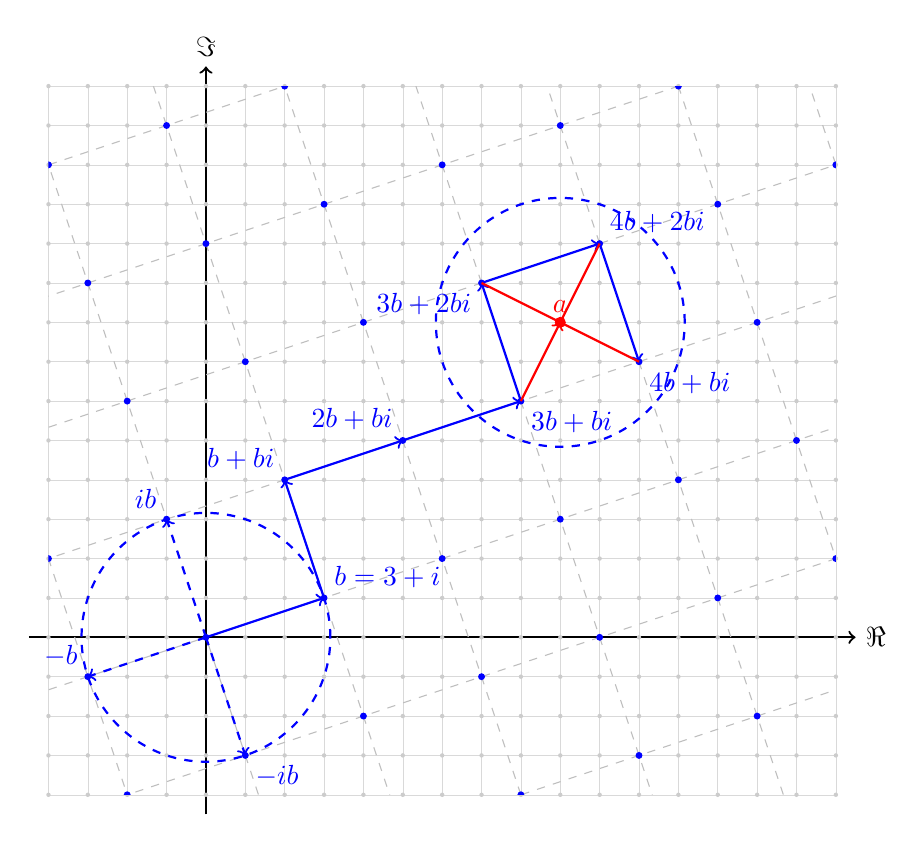
\begin{tikzpicture}[scale=0.5]
      \draw[gray!30, step=1, very thin] (-4,-4) grid (16,14);

      \draw[->, thick] (-4.5, 0) -- (16.5, 0) node[right] {$\Re$};
      \draw[->, thick] (0, -4.5) -- (0, 14.5) node[above] {$\Im$};

      \foreach \x in {-4,...,16} {
        \foreach \y in {-4,...,14} {
          \fill[gray!40] (\x, \y) circle (1.6pt);
        }
      }
      \begin{scope}
        \clip (-4,-4) rectangle (16,14);

        \foreach \m in {-3,...,6} {
          \draw[gray!50, dashed, thin] ({- \m - 30}, {3*\m - 10}) -- ({- \m + 30}, {3*\m + 10});
        }

        \foreach \k in {-3,...,7} {
          \draw[gray!50, dashed, thin] ({3*\k + 10}, {\k - 30}) -- ({3*\k - 10}, {\k + 30});
        }
      \end{scope}

      \begin{scope}
        \clip (-4, -4) rectangle (16, 14);

        \foreach \m in {-5,...,8} {
          \foreach \n in {-5,...,8} {
            \fill[blue] ({3*\m - \n}, {\m + 3*\n}) circle (2.5pt);
          }
        }
      \end{scope}

      \draw[blue, dashed, thick] (0, 0) circle (3.16);
      \draw[blue, dashed, thick] (9, 8) circle (3.16);

      \draw[->, thick, blue] (0, 0) -- (3, 1) node[above right] {$b = 3 + i$};
      \draw[->, thick, dashed, blue] (0, 0) -- (-1, 3) node[above left] {$ib$};
      \draw[->, thick, dashed, blue] (0, 0) -- (-3, -1) node[above left] {$-b$};
      \draw[->, thick, dashed, blue] (0, 0) -- (1, -3) node[below right] {$-ib$};

      \fill[red] (9, 8) circle (4pt) node[above, text=red] {$a$};

      \draw[->, thick, blue] (3, 1) -- (2, 4) node[above left] {$b + bi$};
      \draw[->, thick, blue] (2, 4) -- (5, 5) node[above left] {$2b + bi$};
      \draw[->, thick, blue] (5, 5) -- (8, 6) node[below right] {$3b + bi$};

      \draw[->, thick, blue] (8, 6) -- (7, 9) node[below left] {$3b + 2bi$};
      \draw[->, thick, blue] (7, 9) -- (10, 10) node[above right] {$4b + 2bi$};
      \draw[->, thick, blue] (10, 10) -- (11, 7) node[below right] {$4b + bi$};

      \draw[->, thick, red] (8, 6) -- (9, 8);
      \draw[-, thick, red] (7, 9) -- (9, 8);
      \draw[-, thick, red] (10, 10) -- (9, 8);
      \draw[-, thick, red] (11, 7) -- (9, 8);
    \end{tikzpicture}

    Vemos entonces lo siguiente:

    \begin{equation*}
      \begin{aligned}
        (3 + i)(3 + i) + 1 + 2i &= 9 + 3i + 3i - 1 + 1 + 2i &= 9 + 8i \\
        (3 + i)(3 + 2i) + 2 - i &= 9 + 6i + 3i - 2 + 2 - i  &= 9 + 8i \\
        (3 + i)(4 + 2i) -1 - 2i &= 12 + 6i + 4i - 2 - 1 -2i &= 9 + 8i \\
        (3 + i)(4 + i) -2 + i   &= 12 + 3i + 4i -1 - 2 + i  &= 9 + 8i
      \end{aligned}
    \end{equation*}

    La norma de $b$ es 10, la norma de cualquier residuo de lo vistos anteriormente es 5.
\end{document}
